\chapter{Overview}

Our goal is to enforce low-overhead isolation through memory protection between memory-safe and
memory-unsafe code within a single process, in order to prevent memory corruption vulnerabilities
within memory-unsafe code from violating the integrity of the rest of the application. For example,
this type of sandbox may be used to protect an application from being compromised through a legacy
or 3rd-party library that parses attacker-controlled input and is written in a memory-unsafe
language. Consider a messaging application that uses a vulnerable image decoding library, which an
attacker can exploit by sending a malformed image to the victim: with proper fault isolation, the
attacker may be able to corrupt the decoded image data produced by the library, but they should not
be able to modify unrelated portions of the application's memory, such as the user's contacts or
message history (since that memory should not be accessed when decoding images). This is addressed
effectively by many existing MPK-based sandboxing schemes~\cite{vahldiek-oberwagner:erim,
hedayati:hodor, voulimeneas:cerberus, ghoshn:enclosure}.

Even if memory-unsafe code is protected from writing to protected regions of memory, an attacker may
still be able to indirectly cause corruption of protected memory by exploiting issues on the
boundary between memory-safe and memory-unsafe code. Application developers may misuse complex
sandboxing APIs and fail to correctly restrict memory access permissions when crossing boundaries
between protection domains. This is addressed by automatic sandboxing schemes such as PKRU-safe
\cite{kirth:pkru}, but even the current state-of-the-art schemes cannot enforce that safe code
properly validates sensitive values that are received from unsafe code. For instance, memory-safe
code may dereference an invalid pointer that was received from memory-unsafe code, causing undefined
behavior or memory corruption within memory-safe code that has write access to protected regions of
memory. Thus, we wish to develop a sandboxing scheme that provides a straightforward, safe API to
prevent misuse of the sandbox and improper validation of data exchanged across protection domains.

\section{Security Model}

We assume a program's code is divided into two portions: a "safe" portion written in Rust, and a
"sandboxed" portion written in C or C++. The two portions interact through function calls:
specifically, the safe portion can call functions defined in the sandbox portion. The two portions
can exchange data through function parameters and return values, and by reading and writing data
through pointers returned by these function calls (\autoref{f:sandbox}). Within the scope of our
work, we did not allow calls made in the other direction (C/C++ code calling functions defined in
Rust); additionally, we assume a single-threaded environment.

\begin{figure}[!ht]
    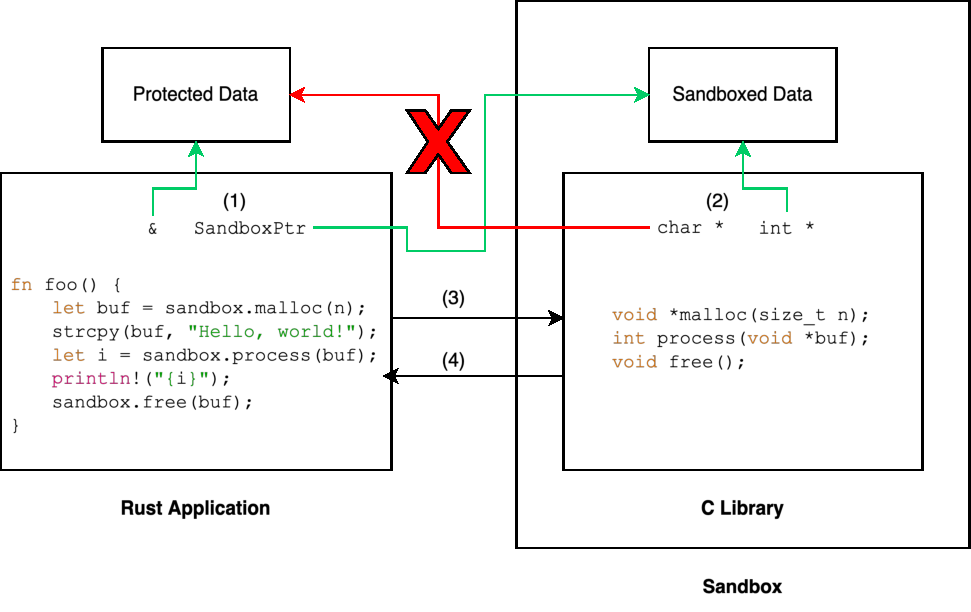
\includegraphics[width=\textwidth]{fig/sandbox}
    \caption[Diagram of our sandbox architecture]{Diagram of our sandbox architecture. Safe Rust
    code is allowed to access its own data (through Rust references) and sandboxed data (through a
    \cc{SandboxPtr} safe pointer type) (1). Unsafe C code can access sandboxed data, but is
    prevented from accessing memory belonging to the safe portion of the program (2). The safe Rust
    code can freely call functions defined in the unsafe portion of the program (3), and the two
    portions can exchange data through parameters and return values (4).}
    \label{f:sandbox}
\end{figure}

We assume the safe portion of our program is free from memory corruption; i.e., that there are no
implementation problems that would cause memory corruption within safe Rust code, and that any
\cc{unsafe} blocks within the Rust code are correctly written and cannot cause undefined behavior.
However, the "sandboxed" portion of our program is expected to contain memory corruption errors
(such as buffer overflows, uninitialized pointers, or use-after-free errors) that an adversary may
be able to exploit with the intent of corrupting variables used by the safe portion of our program.

We wish to define a security model that captures the intuitive idea that an attacker that exploits a
memory corruption vulnerability within sandboxed code can only corrupt memory intended to be
accessed by sandboxed code. This model is not intended to provide absolute security against all possible
memory-corruption attacks, but only on compartmentalization and fault isolation, to mitigate the
access an attacker has to a system after a successful exploit. Additionally, we only consider the
integrity of the application; our definition does not consider attacks on confidentiality (such as
exfiltrating sensitive information from the protected portion of the application) or availability (such
as crashing the application).

We formalize our intuitive model with \autoref{d:isolation}.

\begin{center}
    \centering
    \fbox{\parbox{\textwidth}{
        The sandboxed portion of a program is \textit{isolated} from the secure portion if the
        following conditions hold:
        \squishlist
            \item Memory allocated within safe code cannot be written by sandboxed code.
            \item Memory corruption caused by sandboxed code cannot induce undefined behavior within
                safe code.
        \squishend
    }}
    \captionof{definition}{Isolation}
    \label{d:isolation}
\end{center}

The first condition ensures that a bug in sandboxed code cannot corrupt memory used by unrelated
parts of the program; the second condition ensures that sandboxed code cannot behave in a manner
that could cause safe code to corrupt memory or otherwise behave unexpectedly -- for example, by
returning invalid pointers or values that violate ABI requirements such as alignment or aliasing
guarantees.

This definition is similar to the Biba integrity model~\cite{biba:integrity}. Biba's model asserts
that untrusted code should not be able to write to data owned by trusted code, that trusted code
should not read data owned by untrusted code, and that untrusted code cannot invoke functions
defined in trusted code. Our definition relaxes this second condition: trusted code is allowed to
read untrusted data as long as we can prove that the data is accessed in a manner which cannot cause
memory corruption or other undefined behavior.

Note that our sandbox only considers memory corruption that "escapes" the sandbox. Our work does not
aim to defend against memory corruption that only affects data accessed only within the sandbox, and
it does not aim to defend against attacks that escape the sandbox using means other than memory
corruption -- for example, system calls. An attacker that exploit memory corruption within the
sandbox to make arbitrary system calls could compromise the application without breaking our sandbox
as defined above; thus, to fully secure an application, our memory sandboxing technique must be
combined with a system call sandboxing technique such as mbox \cite{kim:mbox} or Landlock
\cite{linux:landlock}. For the remainder of our paper, we will consider attacks involving
attacker-controlled system calls to be out of scope, even if the attacker is able to gain control
over system calls through memory corruption.

\section{Deny Access or Deny Write?}

One design decision we faced was whether sandboxed code should be permitted read-only access to
protected data, or if protected data should be completely inaccessible. Allowing read-only access
could, in some cases, allow developers to avoid copying data from protected memory into the sandbox,
but it comes at a security disadvantage as sandboxed code could potentially exfiltrate sensitive
information from protected areas of memory.

We decided to choose a security model that only focuses on integrity: \textit{writing} to protected
memory within sandboxed code violates isolation, but reads are allowed. This decision was made to
simplify the implementation: the sandboxed code needs read access to the application memory image
and global offset tables in order to function, so creating a sandbox that protects against write
access would require special-case handling of this memory. (It is not a limitation of our approach;
a straightforward extension of our work would be to use separate protection key to permit read-only
access to non-sensitive data located within the program binary image while denying reads from
sensitive data in the program's data section or heap.) A security model that prevents sandboxed code
from reading from protected memory would contain conditions resembling the Bell-LaPadula
model~\cite{bell:confidentiality}, which describes data confidentiality rather than integrity.
Complete isolation ensuring both confidentiality \textit{and} integrity under both the Biba and
Bell-LaPadula models would prevent interoperability between the safe and sandboxed code entirely (as
the two regions would not be allowed to communicate at all); therefore, we chose to implement a
relaxed Biba integrity model in order to achieve a useful definition of security that allows for a
functional system. 

\section{Enforcing Isolation with Sandboxing}

While the above definitions have made a distinction between sandboxed and safe \textit{code}, we
implement our sandbox by distinguishing between sandboxed and safe \textit{data}. Specifically, we
define all data that is intended to be accessed by sandboxed code as sandboxed data; and all data
that is intended to be accessed solely by safe code as safe data. At every function call into
sandboxed code or returning from such a function, we use the \cc{wrpkru} instruction to restrict or
unrestrict access to safe data accordingly. This instruction modifies the MPK registers to quickly
enable or disable access to regions of memory entirely within userspace, achieving much better
performance than schemes that require invoking the kernel (such as process switching or system calls
such as \cc{mprotect}).

In practice, sandboxed code needs access to any global or static variables defined within that
sandboxed code, but it should not have access to globals defined within safe code. Sandboxed code
needs access to any heap memory that it allocated, but it should not have access to heap memory
allocated by safe Rust code. And sandboxed code needs access to its own stack memory for return
addresses and local variables, but it should not be able to access return addresses and local
variables of safe code.

To achieve this, our work uses memory protection keys to partition the program's address space into
two regions: the "sandboxed" region, which is always accessible by any part of the program, and the
"protected" region, which is accessible to safe code but inaccessible to sandboxed code.

\section{Type-Safely Preventing Undefined Behavior with bindgen}

While the use of memory protection keys as described above is sufficient to achieve the first
condition necessary for isolation, it does not achieve the second. Sandboxed code may return or
write to output parameters values that are illegal under the platform's application binary interface
(ABI), and this induces undefined behavior in safe code that tries to access those values. For
instance:

\squishlist
    \item Sandboxed code may return values that are invalid for the given type -- for example,
        returning a value of boolean type that is neither 0 nor 1.
    \item Sandboxed code may fail to uphold alignment guarantees.
    \item Sandboxed code may return pointers that are null, misaligned, invalid, or point to safe
        memory.
    \item Sandboxed code may return pointers that violate Rust's aliasing and single-mutability
        rules.
\squishend

Rust's \cc{bindgen} "solves" this by marking all generated bindings as \cc{unsafe}: indicating
that invoking them may invoke undefined behavior, and that it is the programmer's responsibility to
verify all relevant memory safety invariants are upheld. Additionally, pointers used as arguments or
return values to C functions are imported to Rust as raw unsafe pointers rather than safe
references; again indicating it is the programmer's responsibility to uphold memory safety when
working with raw pointers.

This is the simplest and most straightforward way of binding to C libraries from Rust programs, and
the semantics are reasonable: when calling into C code, programmers get C's safety guarantees (or
lack thereof). However, we did not consider this an acceptable level of safety for our project. The
complexity of this boundary and the number of invariants it places on the programmer create a high
attack surface, which an attacker with memory corruption within the sandboxed portion of the program
can exploit to induce undefined behavior in the safe portions and pivot to memory corruption there
as well.

Therefore, we modified \cc{bindgen} to provide stronger guarantees in our context of calling into
a sandboxed C library from a Rust program. Notably, we are able to use Rust's type system to express
the requirements and invariants around working with a sandbox, such that we do not need to mark
bindings to sandboxed functions as \cc{unsafe}, and applications can use Rust's safe reference
types to interact with sandboxed data rather than using unsafe raw pointers. Our implementation
transforms all pointer types in C function signatures to safe Rust wrapper types that verify
invariants such as pointer bounds and alignment, and enforce the aliasing requirements needed to
safely interact with sandboxed data using Rust reference types.
